\section{Evaluation}
\label{sec:eval}

We evaluated the characteristics of regression tests in open-source
development from a sample set of Java projects from Github. We are
interested in opportunities to improve performance of test execution
with parallelism \Jbc{Should we use the term parallelism indistinctly
to refer to multi-process and multi-threaded execution?}, measure the
obtained gain (if any), and discuss the major concerns that affect
performance based on the obtained findings.  We pose the following
research questions:

\newcommand{\RQONE}{How prevalent is the occurence of costly
regression tests?}
\newcommand{\rqOne}{\textbf{RQ1.} \RQONE}

\newcommand{\RQTWO}{\Fix{...}}
\newcommand{\rqTwo}{\textbf{RQ2.} \RQTWO{}}

\newcommand{\RQTHREE}{\Fix{...}}
\newcommand{\rqThree}{\textbf{RQ3.} \RQTHREE{}}

\newcommand{\RQFOUR}{How often developers use \Fix{...} to
improve performance on test execution?}
\newcommand{\rqFour}{\textbf{RQ4.} \RQFOUR{}}

\newcommand{\RQFIVE}{\Fix{...}}
\newcommand{\rqFive}{\textbf{RQ5.} \RQFIVE{}}

\begin{itemize}
    \item \rqOne
    \item \rqTwo
    \item \rqThree
    \item \rqFour
    \item \rqFive
\end{itemize}

\Fix{describe what I'm looking for with these RQs}

\subsection{Subjects}
\label{sec:subjects}

We used the Github's Search API to fetch the top 1.000 projects in
Java with at least 100 stars. The number of stars indicates the
interest and appreciation from the community to a given project.
\Comment{(https://help.github.com/articles/about-stars/)} Although our
criteria is subjective, it is an approximation for relevant projects
to conduct our study. For each project, we detected the build manager
system based on the files located in the root directory (\eg,
\emph{pom.xml}) from the project in the following precedence:
\textsc{Maven}, \textsc{Gradle}, and \textsc{Ant}. From the 1.000
downloaded projects, we automatically detected the build system from
806 subjects and selected the \Fix{154} projects that we were able to
compile.  The full list of subjects is publicly available at
\Fix{...}.

\subsection{Answering research question RQ1}
\label{sec:rqone}

\begin{itemize}
    \item \RQONE
\end{itemize}

To evaluate the frequency of costly \Jbc{How to define "costly" in
terms of time?}regression tests, we first compiled the project and
test source files, later, we measured the elapsed time to run the
tests via the build system ignoring non-related tasks (\eg,
\emph{javadoc} generation).  We grouped the resulting time from test
executions in four different groups: tests that ran in less than one
minute (group A), one to five minutes (group B), five to ten minutes
(group C), and more than ten minutes to execute (group D).
Figure~\ref{fig:timecost-barplot} shows the distribution of subjects
per group. It is important to mention that
Figure~\ref{fig:timecost-barplot} represents a lower bound for elapsed
time: since the subjects were tested in a potentially unstable
revision, some tests may fail, interrupting the execution.

\begin{figure}[t!]
    \centering
    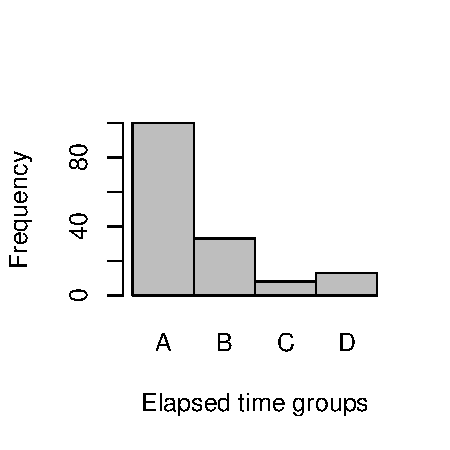
\includegraphics[width=0.5\textwidth]{plots/timecost-barplot/timecost-barplot.pdf}
    \caption{\label{fig:timecost-barplot} \Fix{Subjects grouped by
        elapsed time on test execution ($t$): group A ($t < 1m$), group B
        ($1m \leq t < 5m$), group C ($5m \leq t < 10m$), group D ($10m \leq t$)}}
\end{figure}

\begin{figure}[t!]
    \centering
    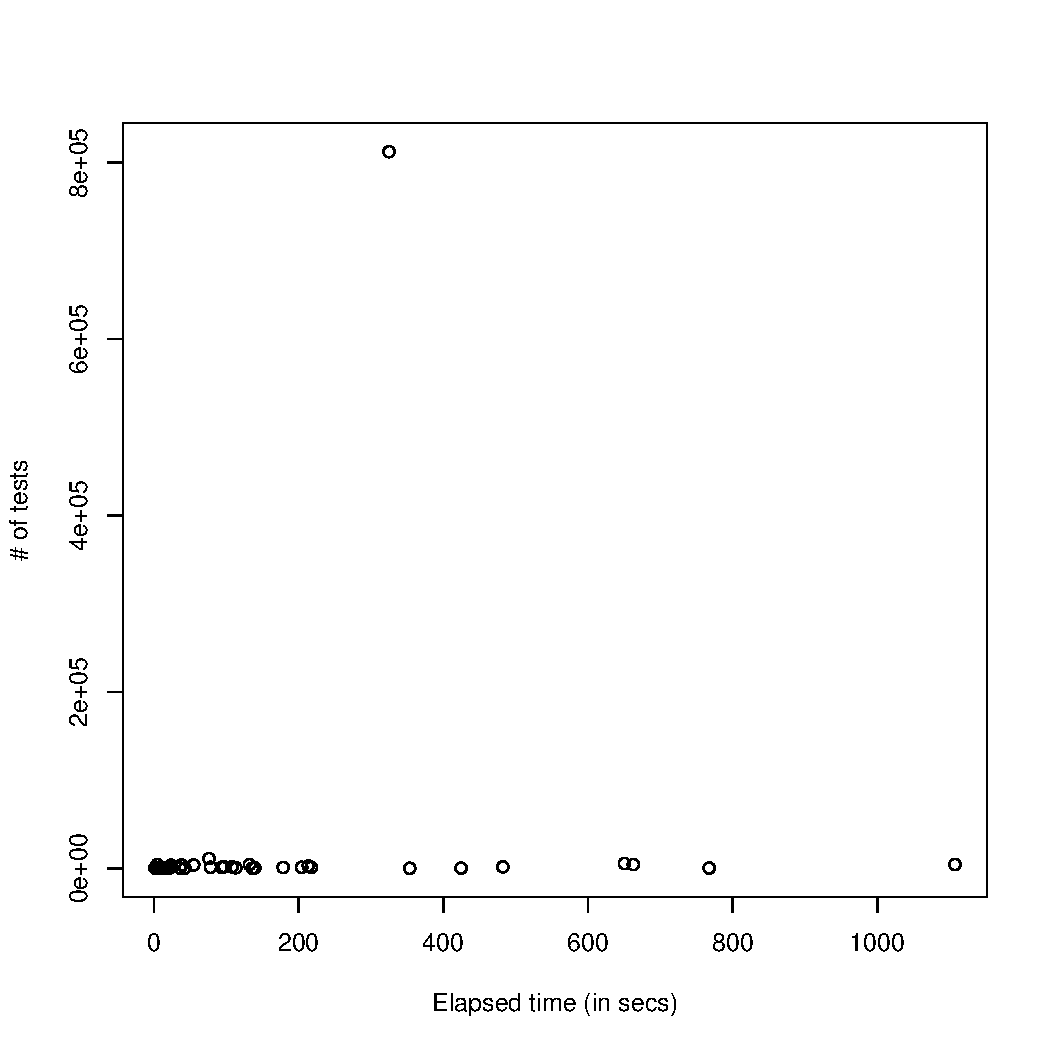
\includegraphics[width=0.5\textwidth]{plots/teststime-scatter/timetests-scatter.pdf}
    \caption{\label{fig:timetests-scatter} \Fix{...}}
\end{figure}
